\documentclass[letterpaper]{article}
\title{CSE 546 Machine Learning, Autumn 2013 \\ Homework 2 \\ Shrainik Jain - 1323338}
\date{}
\usepackage{hyperref}

\usepackage[margin=1.5in]{geometry}

\usepackage{amsmath,amsfonts}
\usepackage{capt-of}
\usepackage{url}
\usepackage{graphicx}
\usepackage{color}
\usepackage{bbm}
\usepackage{enumerate}
\newcommand{\carlos}[1]{\textcolor{red}{Carlos: #1}}
\newcommand{\field}[1]{\mathbb{#1}} 
\newcommand{\hide}[1]{#1}
\newcommand{\pd}[2]{\frac{\partial #1}{\partial #2}}
\providecommand{\m}[1]{\mathbf{#1}}
\providecommand{\norm}[1]{\left\|#1\right\|}
\providecommand{\sign}[1]{\text{sign}\left(#1\right)}
\DeclareMathOperator*{\argmin}{arg\,min}
\providecommand{\what}{\m{\hat{w}}}

\begin{document}

\maketitle
\section{Boosting} 
%
%
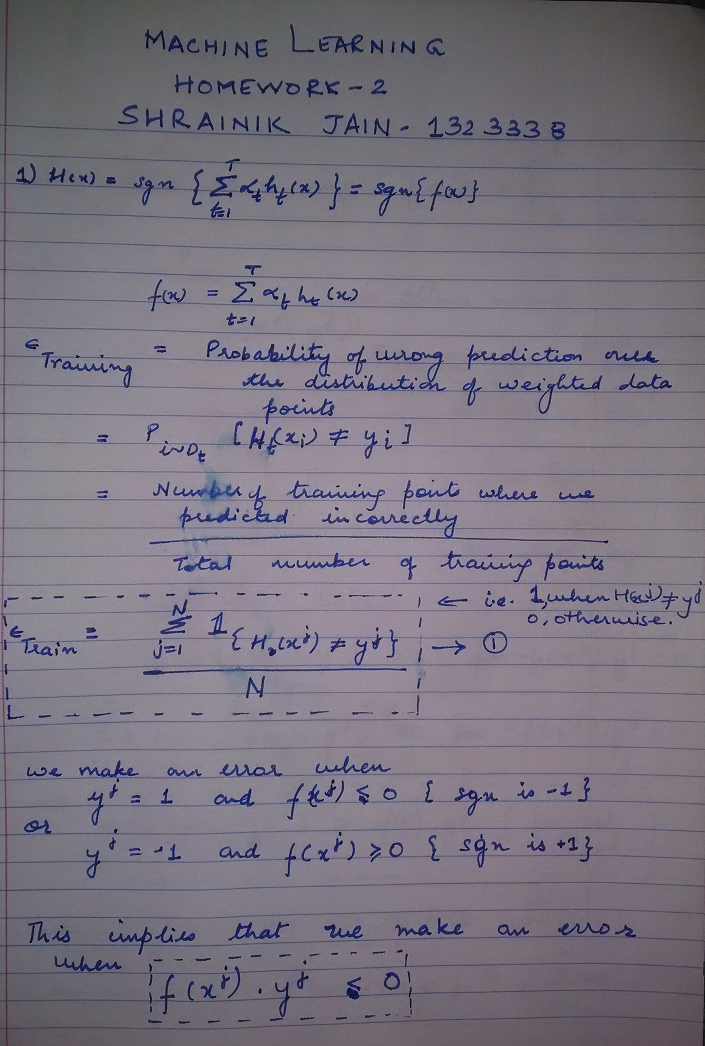
\includegraphics[width = 5.9in, height = 7.5in]{1.png}
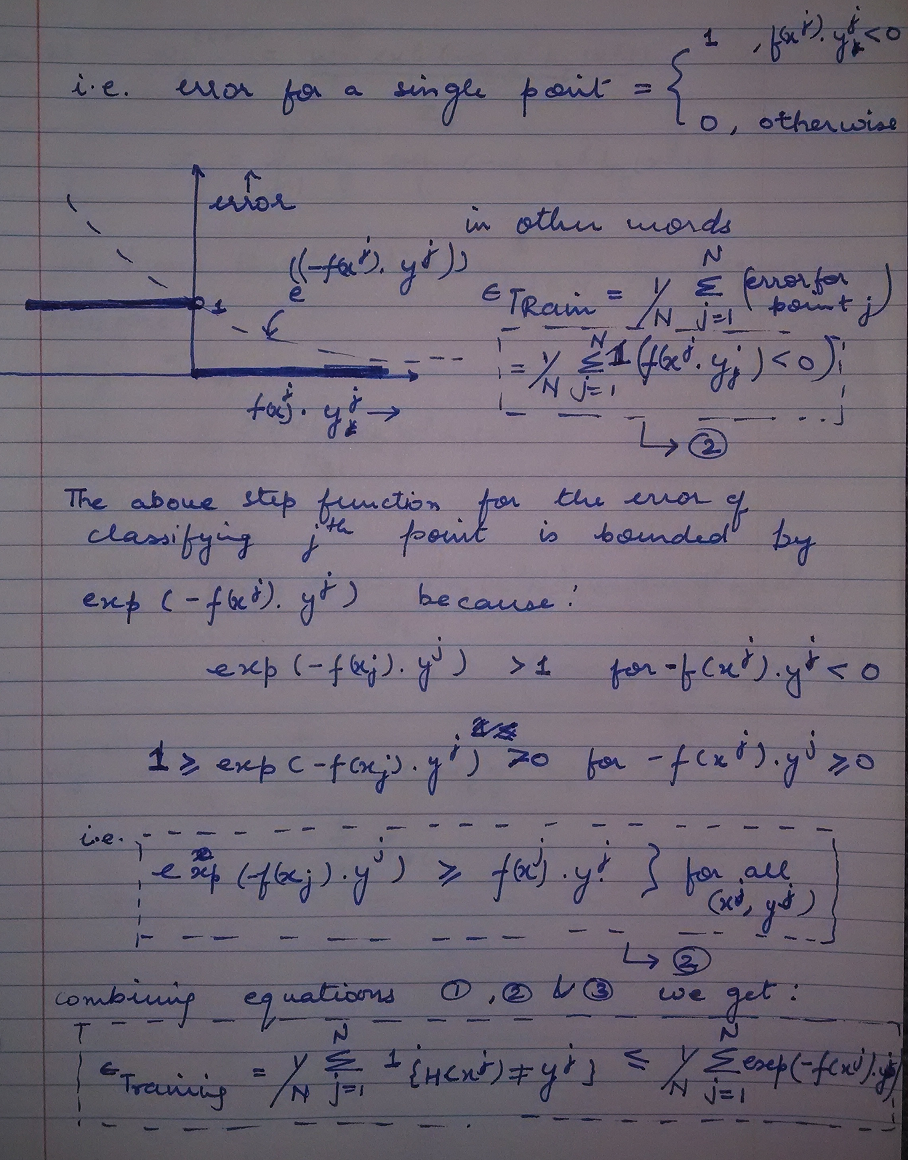
\includegraphics[width = 6in]{2.png}
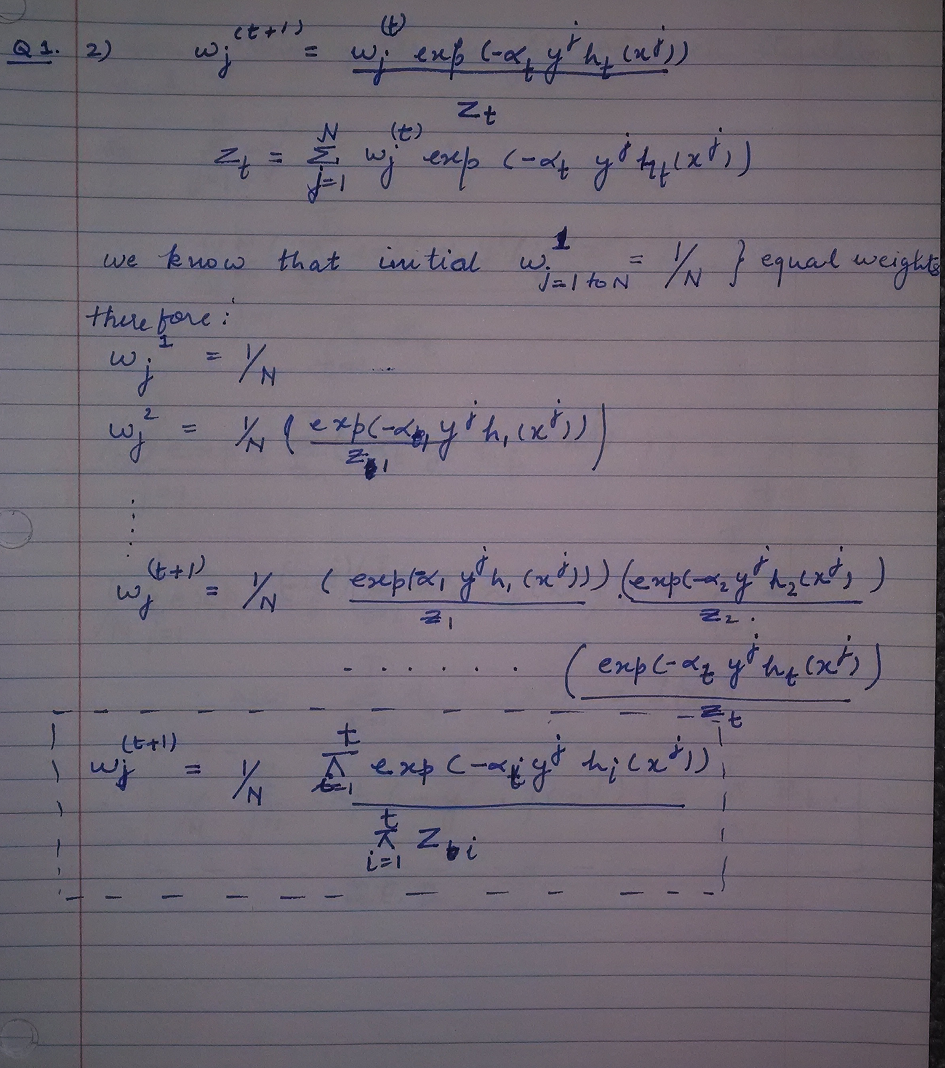
\includegraphics[width = 6in]{3.png}
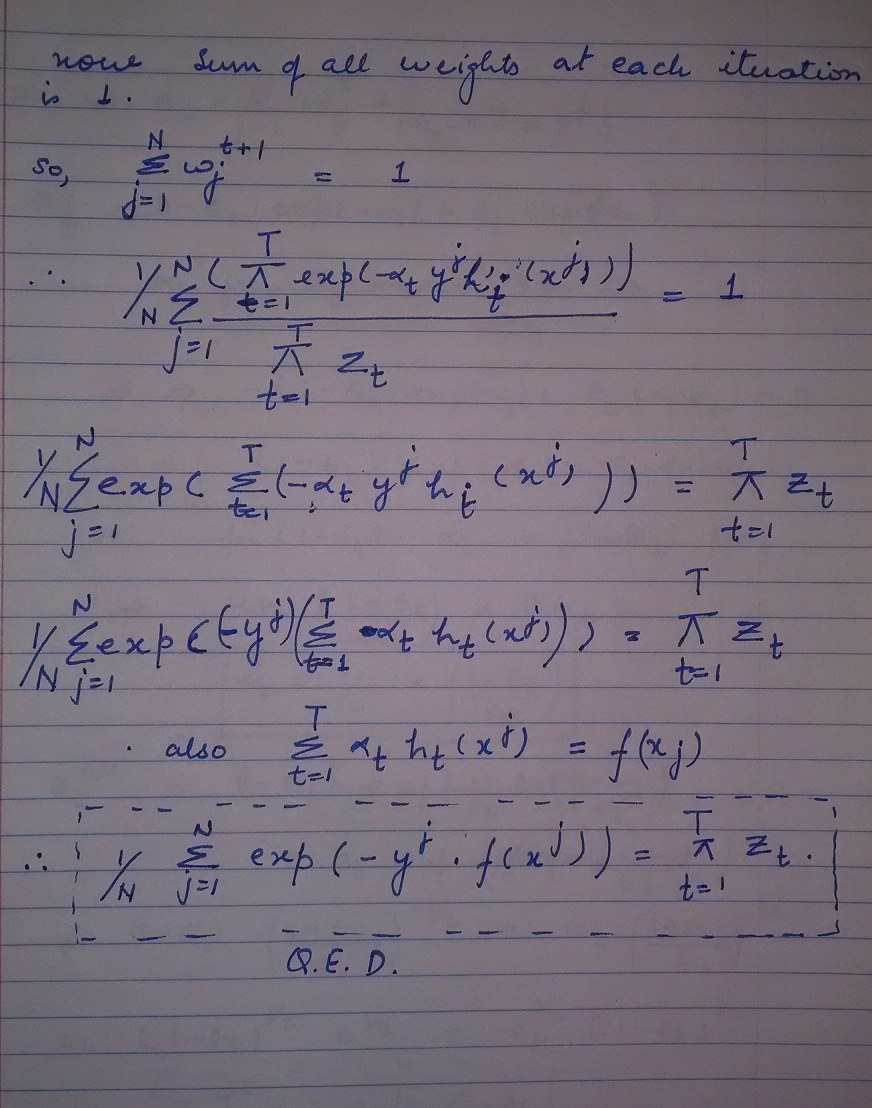
\includegraphics[width = 6in]{4.png}
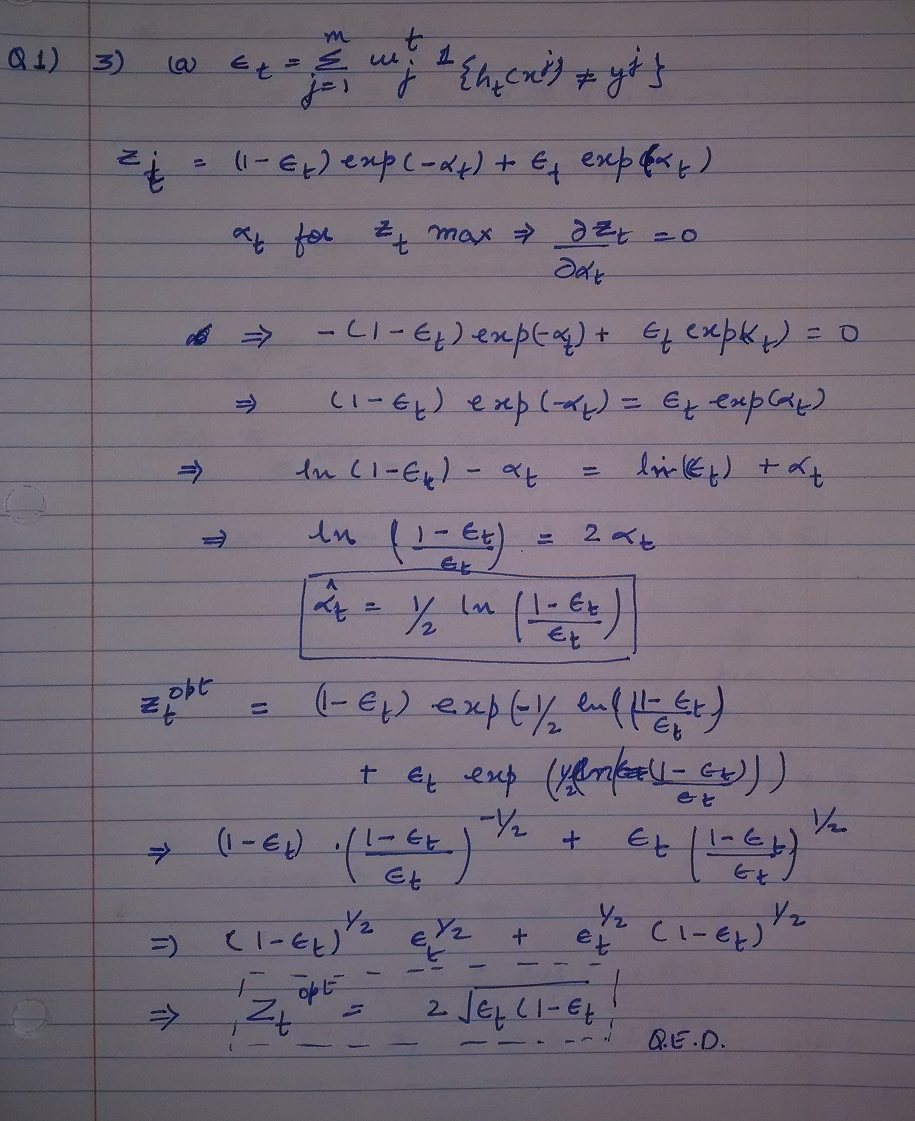
\includegraphics[width = 6in]{5.png}
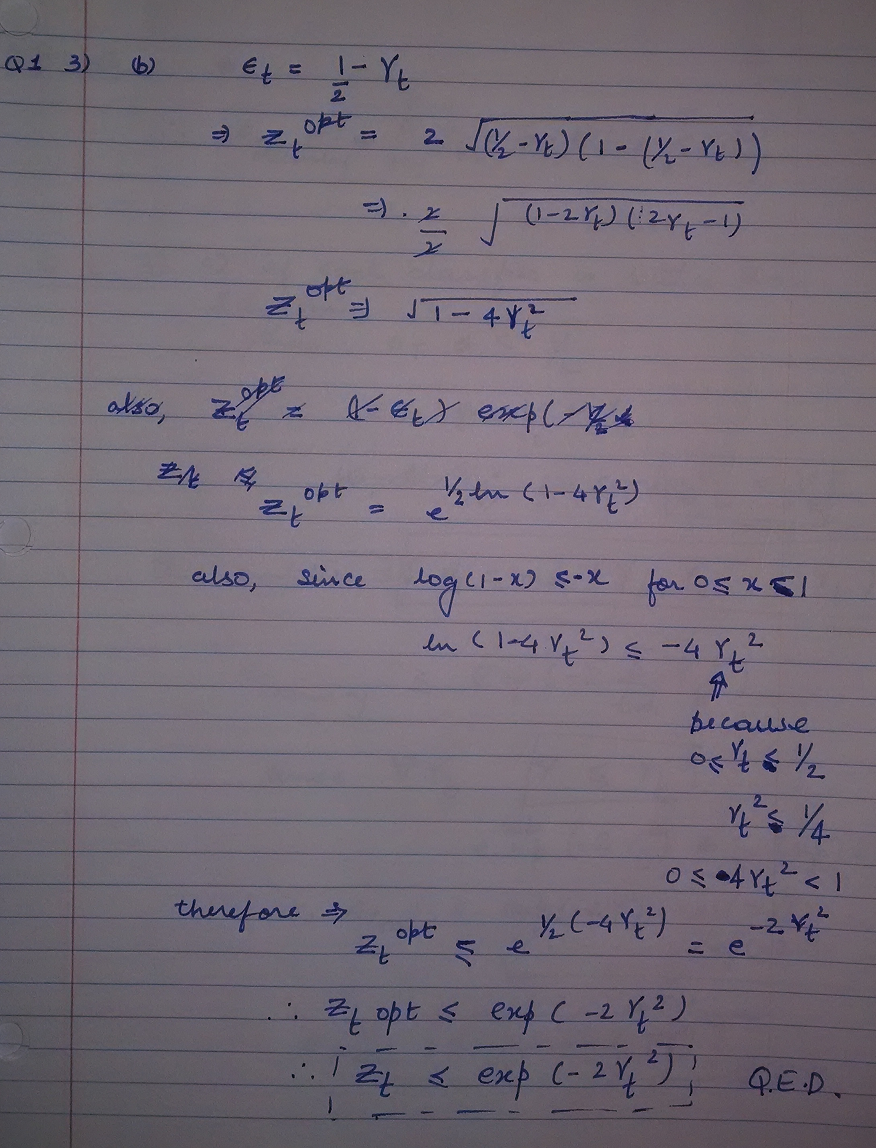
\includegraphics[width = 6in]{6.png}
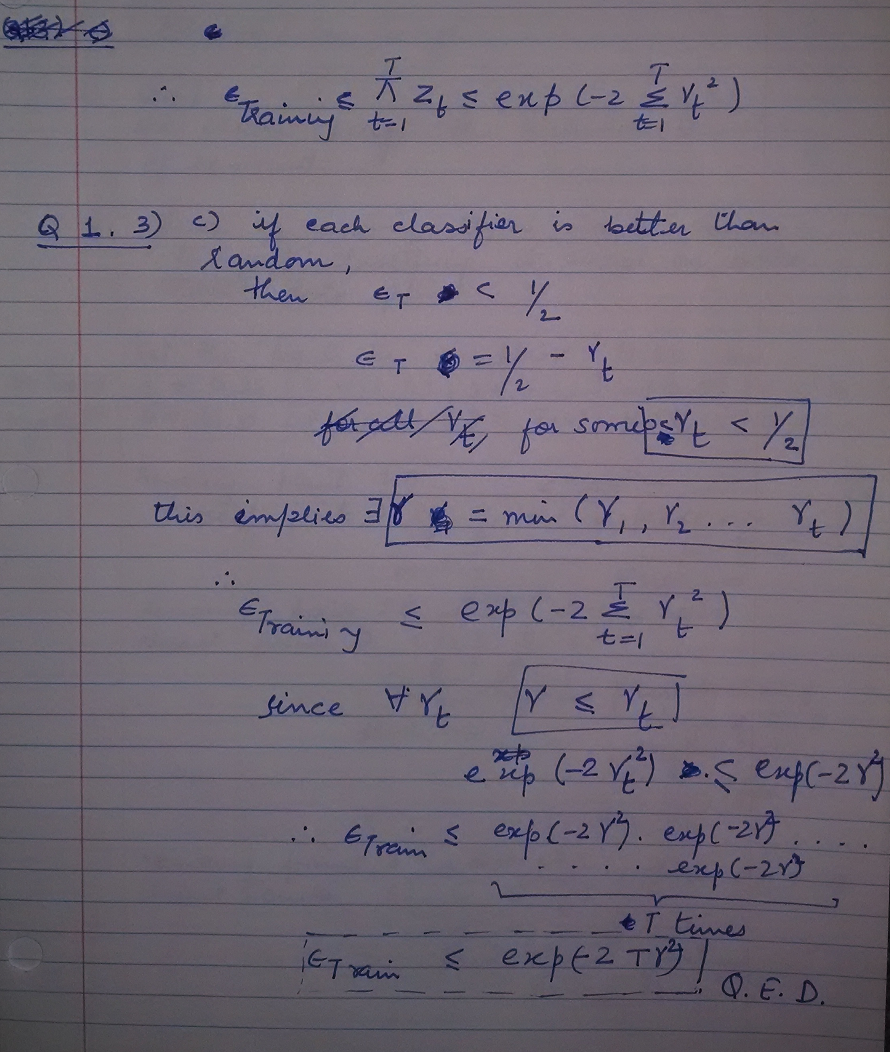
\includegraphics[width = 6in]{7.png}

\section{KNN}
The following figure is the Voronoi diagram for the dataset. The Redline is the decision boundary, i.e. all points left of it are positive.
\begin{center}
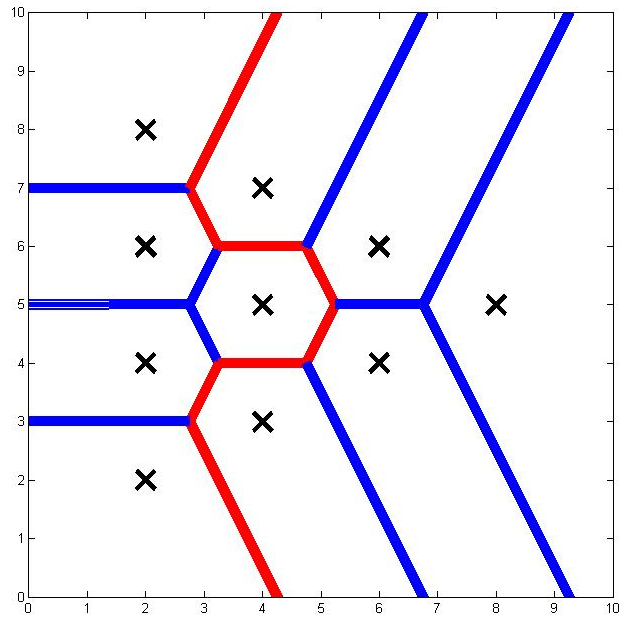
\includegraphics[width = 4in]{8.png}
\end{center}
\begin{center}
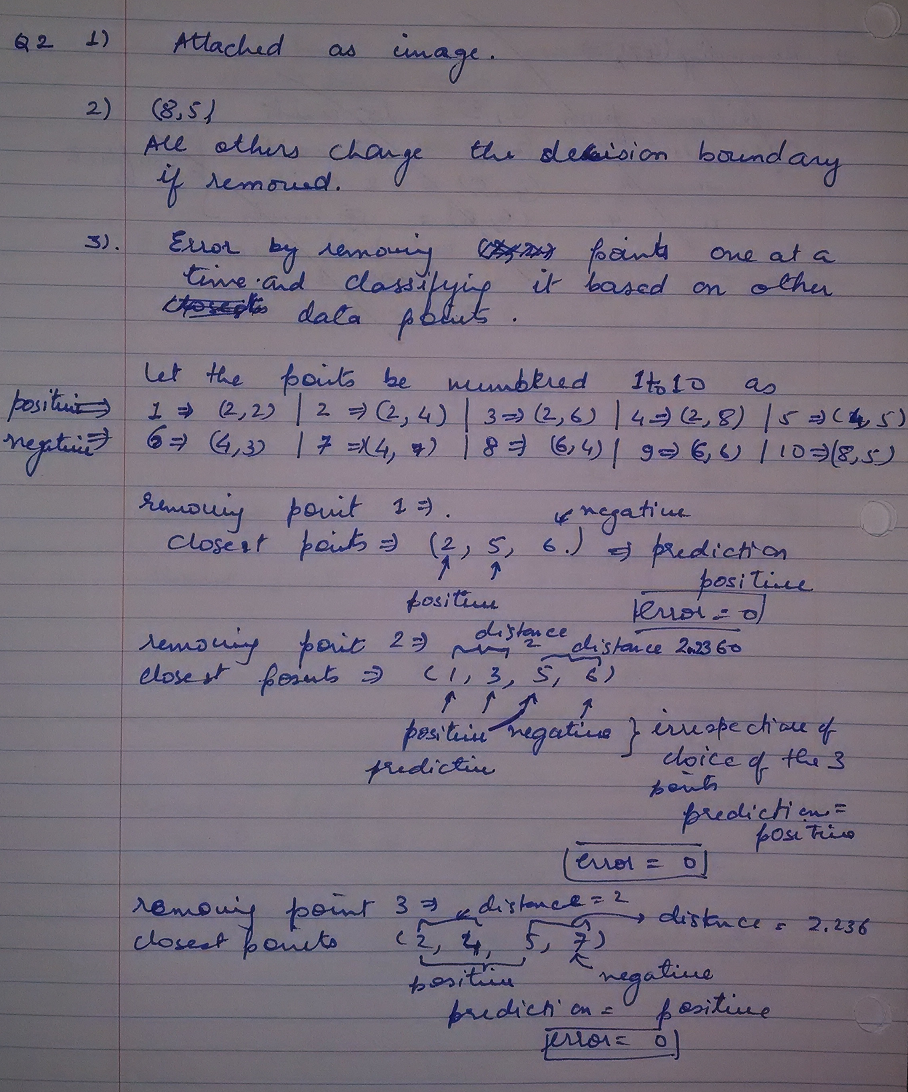
\includegraphics[width = 6in]{9.png}
\end{center}

\begin{center}
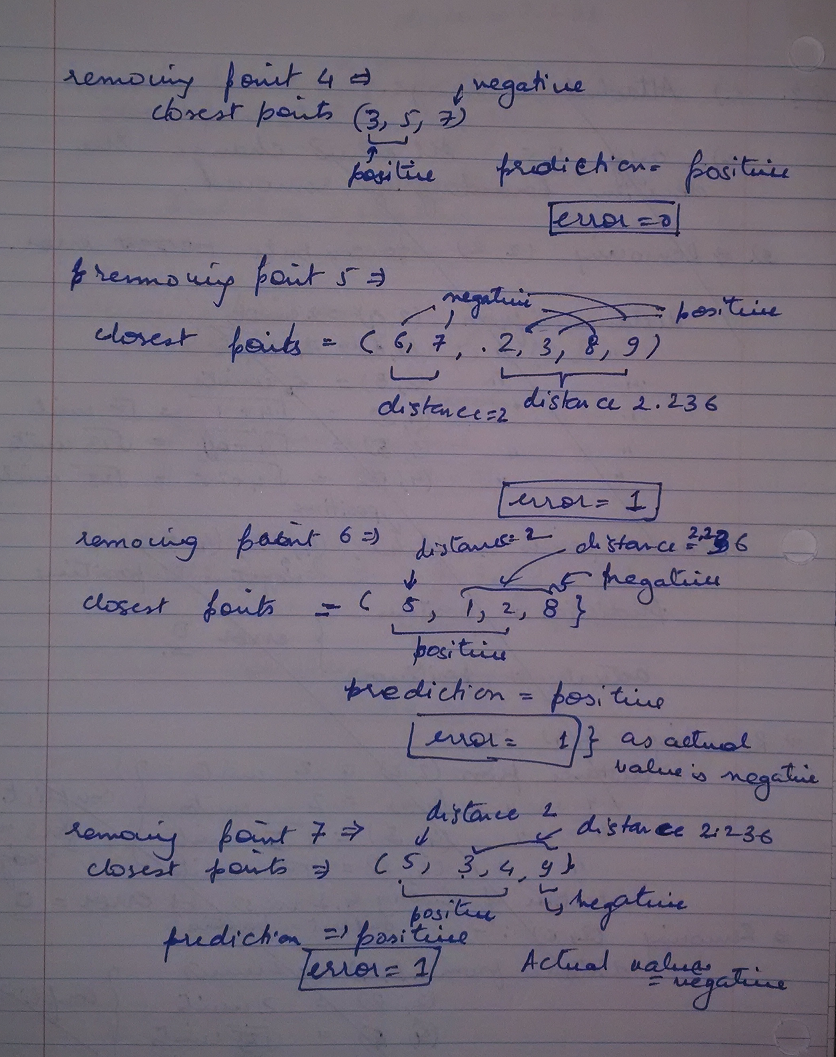
\includegraphics[width = 6in]{10.png}
\end{center}

\begin{center}
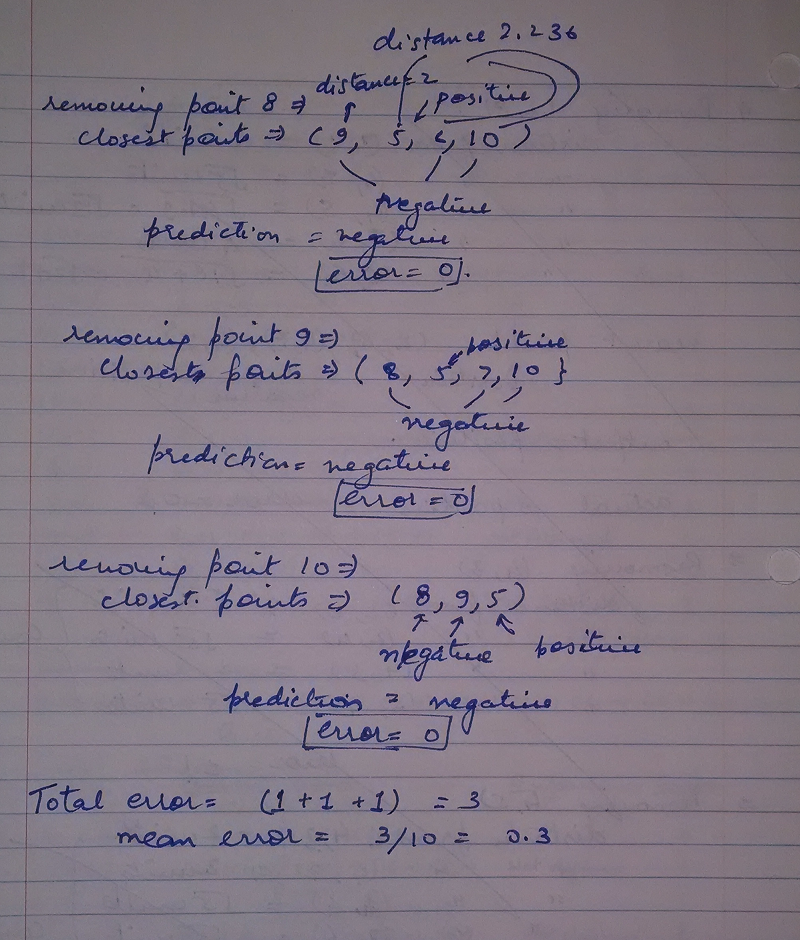
\includegraphics[width = 6in]{11.png}
\end{center}

\begin{center}
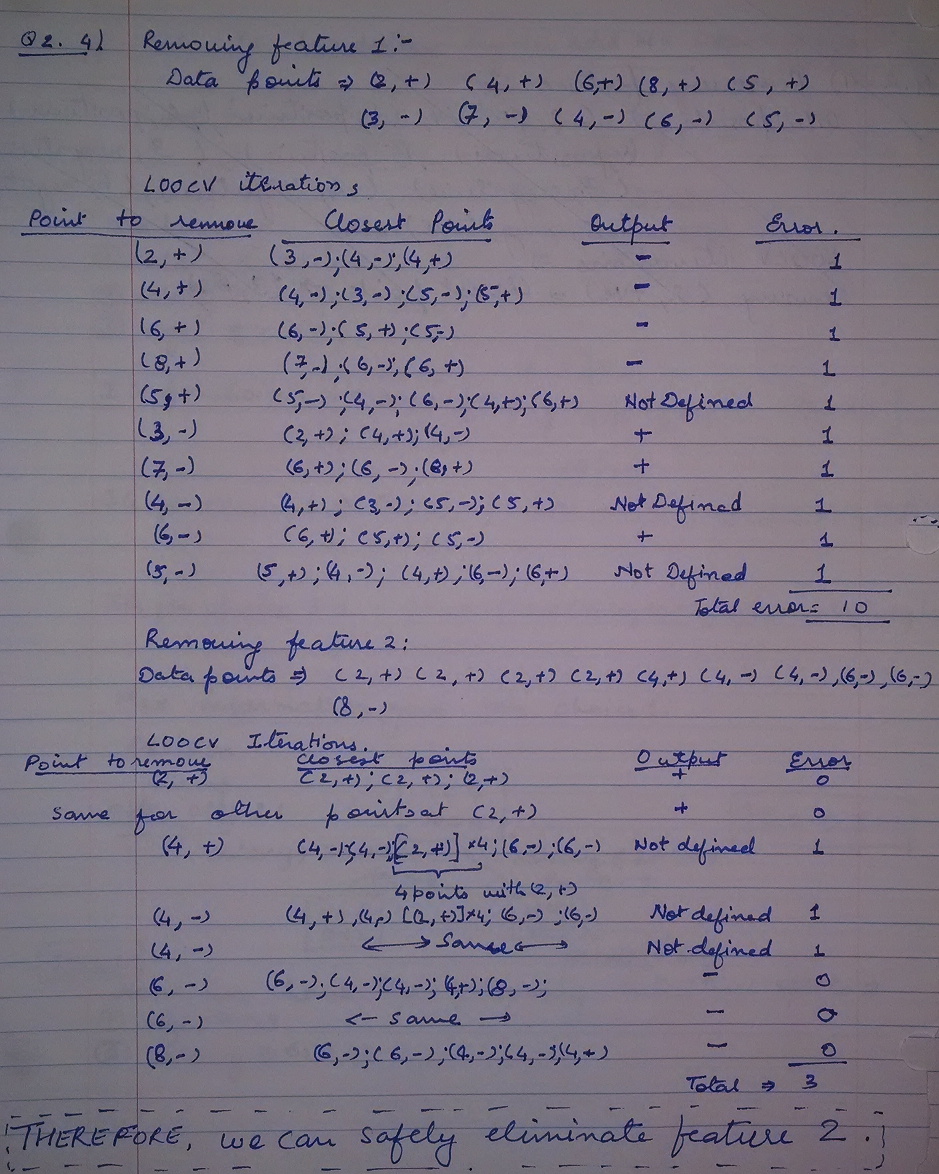
\includegraphics[width = 6in]{12.png}
\end{center}

\section{Decision Trees}
\subsection{}
\begin{center}
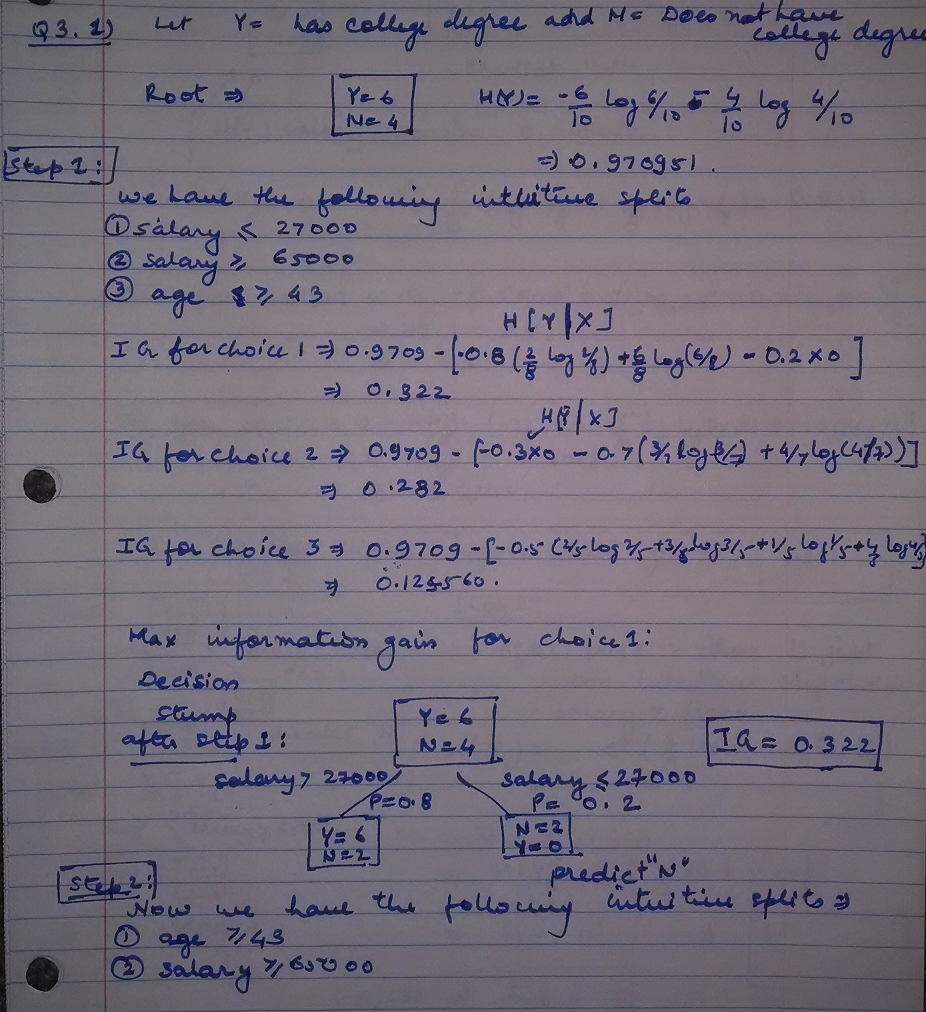
\includegraphics[width = 6in]{13.png}
\end{center}

\begin{center}
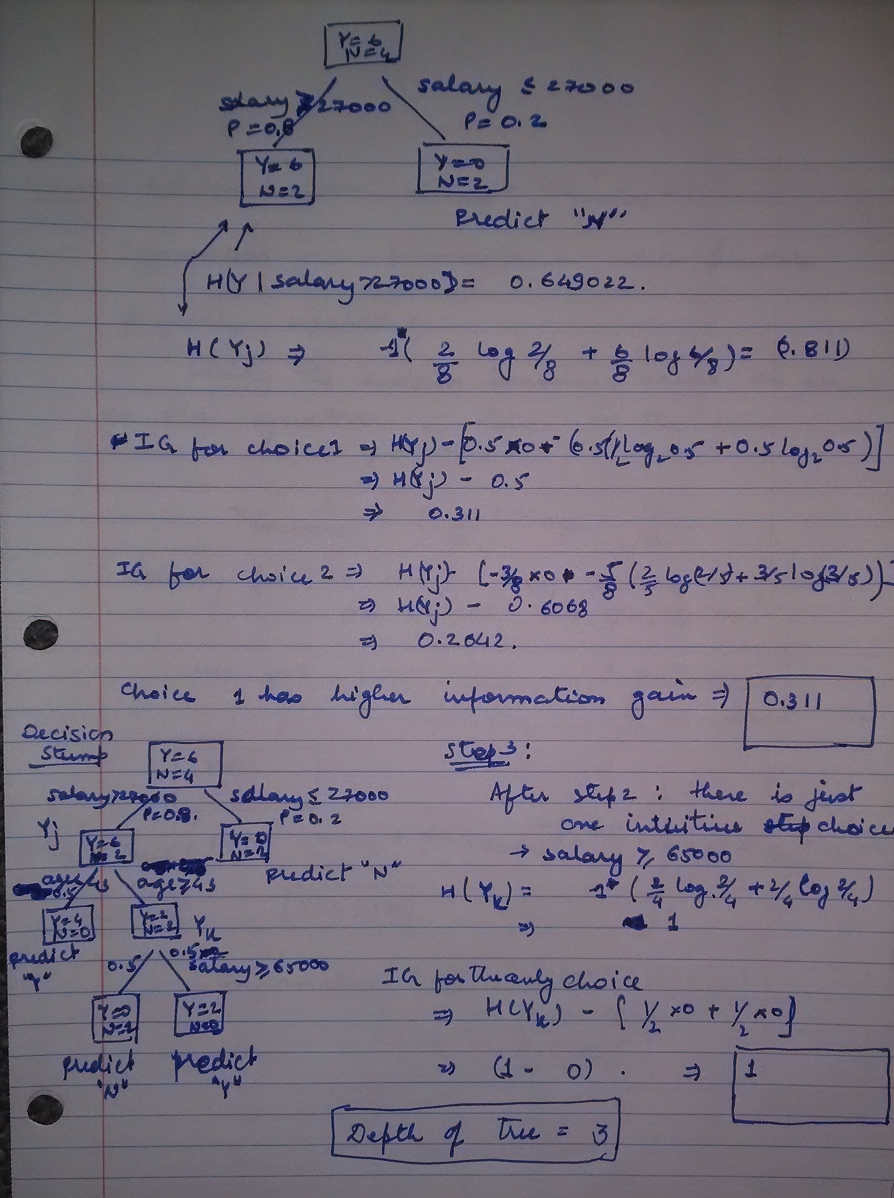
\includegraphics[width = 6in]{14.png}
\end{center}
\subsection{}
\begin{center}
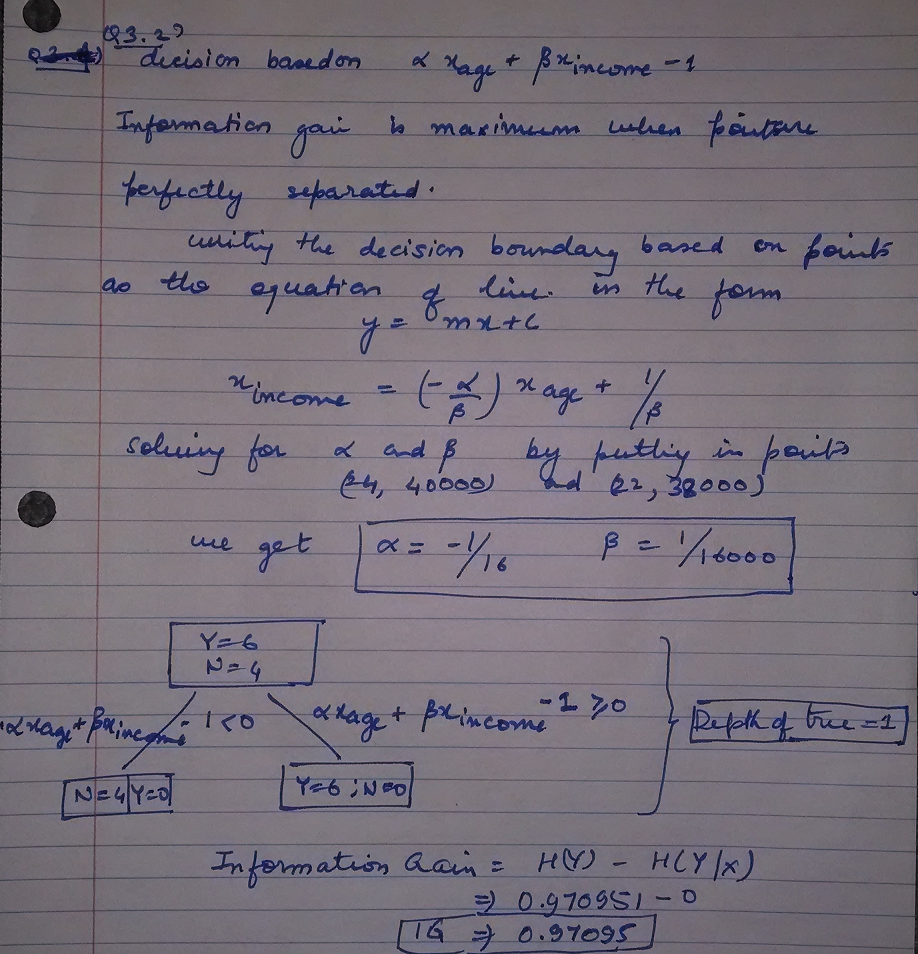
\includegraphics[width = 6in]{15.png}
\end{center}
\subsection{}
Advantages of multivariate decision trees:
\begin{itemize}
\item	More than one feature can be tested for per decision, this helps getting a way better predictor when the data points are linearly separable.
\item	Training error is lower as more complex models are allowed (decision based on multiple variables and rather than a single variable).
\item	Multivariate decision trees will have, on an average, smaller tree size. 
\end{itemize}

Disadvantages of multivariate decision trees:
\begin{itemize}
\item	The computation cost (CPU Time) of the learning algorithm is very high (imagine running linear regression again and again for each decision node), as a lot of features need to be tested to find out the maximum information gain per step. While the univariate algorithm requires considering only one feature at a time.
\item	On smaller datasets, multivariate trees tend to over-fit a lot because of standard deviation in the data points. This leads to higher test errors. Multivariate trees require a lot of data-points which might or might not be present.
\end{itemize}

\section{Programming Question}

\subsection{Unprocessed Dataset}
No question in this part.

\subsection{Processed Dataset (that you will use...)}
No question in this part.

\subsection{Accessing and Processing the Data}
No question in this part.

\subsection{Batch Gradient Descent}

\begin{enumerate}
\item Actual weight update step: 
\begin{equation}
w^{t+1}_i = w^t_i + \eta(-\lambda w^t_i + \sum_{j=1}^N{x^j_i(y^j - \frac{e^{w_0 + \sum{w_ix^j_i}}}{1 + e^{w_0 + \sum{w_ix^j_i}}})})
\end{equation}
Weight update step in python: 
\begin{verbatim}
#(Y is Nx1, X is Nx(D+1), W is (D+1)x1)

yj_minus_p = Y - (exp(X.dot(W))/(1+ exp(X.dot(W))))
W[0] = W[0] + (eta / N) * sum(yj_minus_p)
W[1:] = (1 - eta * lmbd) * W[1:] + eta * (array(yj_minus_p).dot(X[:,1:]) / N)
\end{verbatim}
\item 
\begin{enumerate}
\item Log loss versus number of iterations: 
\begin{center}
 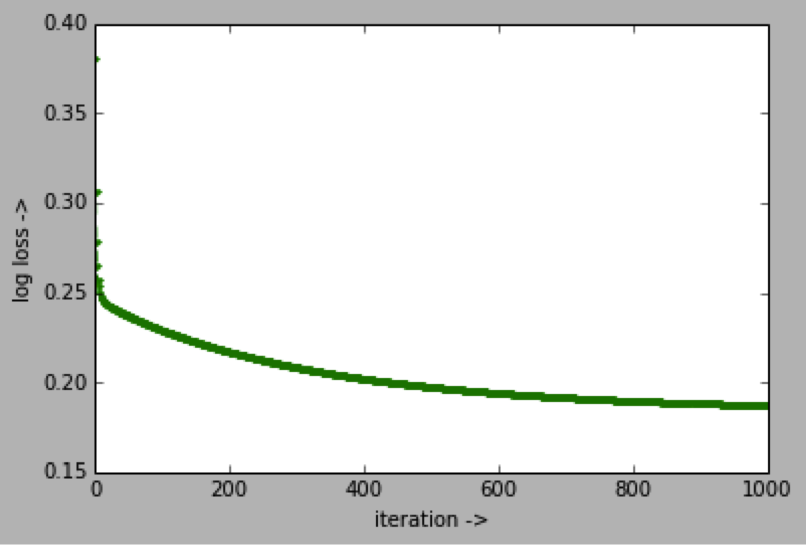
\includegraphics[width=3.5in]{log_loss1.png}
\end{center}
\item SSE for batch gradient descent with 1000 iterations: 54.0
\end{enumerate}
\item 
\begin{enumerate}
\item Number of iterations with the stopping criteria: 13
\item Log loss versus Iterations for gradient descent with the stop criteria:
\begin{center}
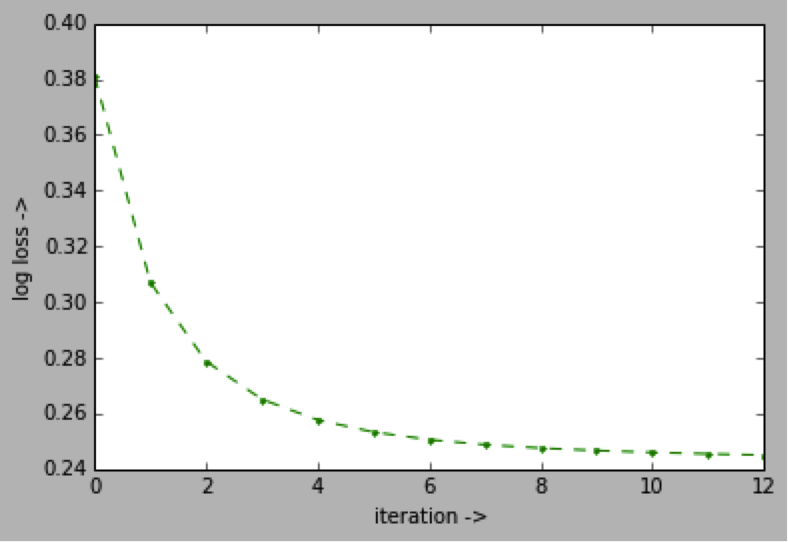
\includegraphics[width=3.5in]{log_loss2.png}
\end{center}
\item SSE for batch gradient descent with the stop criteria: 54.0
\end{enumerate}

\end{enumerate}


\subsection{Stochastic Gradient Descent}

\begin{enumerate}
\item Actual weight update step: 
\begin{equation}
w^{t+1}_i = w^t_i + \eta(-\lambda w^t_i + x^j_i(y^j - \frac{e^{w_0 + \sum{w_ix^j_i}}}{1 + e^{w_0 + \sum{w_ix^j_i}}}))
\end{equation}
Weight update step in python: 
\begin{verbatim}
#(Y is Nx1, X is Nx(D+1), W is (D+1)x1)

yj_minus_p = Y[j] - (1-1/(1+exp(X[j,:].dot(W))))
W[0] = W[0] + (eta) * yj_minus_p
W[1:] = (1 - eta * lmbd) * W[1:] + eta * (yj_minus_p * (X[j,1:]))
\end{verbatim}
\item 
\begin{enumerate}
\item $l_2$ norm for:
\begin{itemize}
\item $\lambda = 0$ : 1.92503456434
\item $\lambda = 0.3$ : 0.283520413611
\end{itemize} 
\item SSE for $\lambda = 0.3$ : 54.0
\item Feature weights for:
\begin{itemize}
\item $INTERCEPT$ : -3.10616785425 
\item $DEPTH$:  0.109353101677
\item $POSITION$: -0.006094751226
\end{itemize}
\end{enumerate}

\item After 5 iterations, log loss with:
\begin{itemize}
\item Stochastic Descent: 0.197392978738
\item Gradient Descent: 0.257743788383
\end{itemize}
Stochastic Descent seems to converge faster.
\end{enumerate}

\subsection{Class Imbalance}

\begin{enumerate}
\item For predictions made by SGD running with one pass over data, and $\lambda = 0.3$ and $\eta = 0.1$:
\begin{itemize}
\item Precision and Recall for class 0: 0.946, 1.0
\item Precision and Recall for class 1: 0.0, 0.0
\end{itemize}

\item For predictions made by batch gradient descent running for 10000 iterations over the oversampled data and with $\lambda = 0.3$ and $\eta = 0.01$:
\begin{itemize}
\item Precision and Recall for class 0: 0.94140625, 0.509513742
\item Precision and Recall for class 1: 0.04918032, 0.444444444
\end{itemize}
\end{enumerate}

\end{document}
